\documentclass{ltjsarticle}
\usepackage{amsmath,amssymb,amsthm}
\usepackage{mathcomp}
\usepackage{graphicx,color}
\usepackage{verbatim}
\usepackage{tikz}
\usepackage{luatexja-ruby}
\usepackage[pdfusetitle]{hyperref}
\title{たのしい複素積分}
\author{荒田 実樹}

\usetikzlibrary{arrows.meta,decorations.pathreplacing,decorations.markings,shapes.misc,patterns}

\newcommand{\Natural}{\mathbf{N}}
\newcommand{\Integer}{\mathbf{Z}}
\newcommand{\Real}{\mathbf{R}}
\newcommand{\Complex}{\mathbf{C}}
\newcommand{\ImagI}{i}%{\sqrt{-1}}%{\mathbf{i}}
\newcommand{\innerProd}[2]{\left\langle #1,#2\right\rangle}
\newcommand{\norm}[1]{\left\lvert #1\right\rvert}
\newcommand{\abs}[1]{\left\lvert #1\right\rvert}
\DeclareMathOperator{\RealPart}{Re}
\DeclareMathOperator{\ImagPart}{Im}
\DeclareMathOperator{\Residue}{Res}

\theoremstyle{definition}
\newtheorem{theorem}{定理}
\newtheorem{lemma}[theorem]{Lemma}
\newtheorem*{lemma*}{Lemma}
\newtheorem{proposition}[theorem]{Proposition}
\newtheorem*{proposition*}{Proposition}
\newtheorem{cor}[theorem]{Corollary}
\newtheorem*{cor*}{Corollary}
\newtheorem{fact}[theorem]{Fact}
\newtheorem*{fact*}{Fact}
\newtheorem{definition}{Definition}
\newtheorem*{definition*}{Definition}

\theoremstyle{remark}
\newtheorem{remark}[definition]{Remark}
\newtheorem*{remark*}{Remark}
\newtheorem{claim}{Claim}
\newtheorem*{claim*}{Claim}
\newtheorem{example}{例}
\newtheorem*{example*}{Example}
\newtheorem{exercise}[example]{問題}

\begin{document}
%\maketitle

\Chapter{たのしい複素積分(荒田)}

\Section{はじめに}

数ヶ月前のことですが,複素積分で遊べるWebページを作りました.
以下のURLからアクセスできます.URLを打ち込むのが面倒な人はQRコードを読み取ってください.
あるいは,「たのしい複素積分」でググったら出てくるかもしれません.

\begin{center}
\url{http://d-poppo.nazo.cc/math/singularity/} \\
\includegraphics[width=3cm]{arata-qrcode.eps}
\end{center}

この記事では,複素積分ってなにそれおいしいの?という人のために複素解析のさわりを紹介します.
諸概念の厳密な定義とか定理の証明とかはここではしないので,複素解析の教科書を読んでください.

複素解析の教科書としては,Ahlforsによる教科書\cite{Ahlfors} が定番でしょう.
邦訳\cite{Ahlfors-ja} もあります.
高校生や大学初年度向けの入門書として,『複素数の世界』\cite{Ueno} も挙げておきます.
図書館で探してみると良いでしょう.

以下では,読者は,複素数の基本的な性質及び,実数の微積分についてはある程度知っているものとします.
%高校生 $+\alpha$ ぐらいの知識で読めるといいな

\newcommand{\exampleautorefname}{例}

\Section{複素関数}
複素数に複素数を対応させる関数 $f\colon\Complex\to\Complex$ を複素関数と呼びます.
正確には,複素平面全体で定義されている必要はなくて,複素平面の一部分で定義されていれば複素関数と呼びます(\autoref{example:1/z} など).

複素数は2つの実数の組と思えますが,それと同じように,複素関数 $f(z)$ は,2変数の実関数 $u(x,y)$, $v(x,y)$ を組み合わせたものと見ることもできます.
\[f(x+\ImagI y)=u(x,y)+\ImagI v(x,y)\]

% 図
%\begin{center}
%  \begin{tikzpicture}
%    \draw [-{Stealth}] (-2,0) -- (2,0);
%    \draw [-{Stealth}] (0,-2) -- (0,2);
%    \draw plot [smooth cycle, tension=1] coordinates {(-1,-0.9) (-0.3,-0.8) (0.7,-0.9) (1.3,0.3) (0.8,1) (0.1,0.8) (-0.7,1.2) (-1,0.3) (-0.9,-0.2)};
%  \end{tikzpicture}
%\end{center}

いくつかの複素関数について,その実部 $u(x,y)$ と虚部 $v(x,y)$ を見てみましょう.

\begin{example}
  $f(z)=z^2+1$ という関数について,
  %\[
  %f(x+\ImagI y)
  %=(x+\ImagI y)^2+1
  %=x^2+2\ImagI xy-y^2+1
  %\]
  %より
  \[u(x,y)=x^2-y^2+1, \quad v(x,y)=2xy.\]
  %である.
\end{example}

\begin{example}
  指数関数 $f(z)=\exp z$ について,%の $u$, $v$ は
  \[u(x,y)=e^x\cos y, \quad v(x,y)=e^x\sin y.\]
\end{example}

\begin{example} \label{example:1/z}
  複素数の逆数をとる関数 $f(z)=\frac{1}{z}$ は,複素平面から原点 $0$ を除いた部分で定義される.
  この関数について,実部と虚部は
  \[u(x,y)=\frac{x}{x^2+y^2}, \quad v(x,y)=-\frac{y}{x^2+y^2}.\]
\end{example}

\begin{example}
  複素数の実部をとる関数 $f(z)=\RealPart z$ について,
  \[u(x,y)=x, \quad v(x,y)=0.\]
\end{example}

\begin{example}
  複素共役をとる関数 $f(z)=\bar{z}$ について,
  \[u(x,y)=x, \quad v(x,y)=-y.\]
\end{example}


\Section{複素微分と正則関数}
\newcommand{\pdiff}[2]{\frac{\partial #1}{\partial #2}}

複素積分の話に入る前に,複素関数の微分を定義しておきます.
点 $z=z_0$ のまわりで定義された複素関数 $f$ について,極限
\[\lim_{h\to 0} \frac{f(z_0+h)-f(z_0)}{h}\]
が存在するとき, $f$ は点 $z_0$ で複素微分可能であるといいます.
このとき,$f$ の $z=z_0$ における微分係数 $f'(z_0)$ を,その極限値
\[f'(z_0):=\lim_{h\to 0} \frac{f(z_0+h)-f(z_0)}{h}\]
として定義します.
定義域のいたるところで複素微分できる関数を\ruby{正則}{せいそく}関数(holomorphic function)と呼びます.

一見すると変数が実数のときの微分と同じ定義ですが,実数の場合は $h$ が左から近づくか右からかぐらいしか $0$ への近づき方がなかったのに対し,ここでの $h$ は上下左右どの方向からでも $0$ に近づいても良いという点が違います.
このことによって,複素関数が微分できるという条件は,対応する実数の関数 $u$, $v$ が(実数の意味で)微分可能である,という条件よりも強い条件となっています.

% 近づき方の図
\begin{center}
  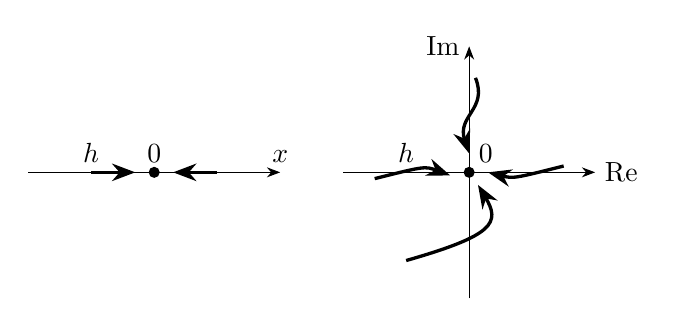
\begin{tikzpicture}[x=0.8cm,y=0.8cm]
    \begin{scope}[xshift=-2cm]
      \draw [-{Stealth}] (-2,0) -- (2,0) node [above] {$x$};
      \draw [-{Stealth},very thick] (-1,0) -- (-0.3,0);
      \fill (0,0) circle (2pt) node [above] {$0$};
      \draw [-{Stealth},very thick] (1,0) -- (0.3,0);
      \node [above] at (-1,0) {$h$};
    \end{scope}
    \begin{scope}[xshift=2cm]
      \draw [-{Stealth}] (-2,0) -- (2,0) node [right] {Re};
      \draw [-{Stealth}] (0,-2) -- (0,2) node [left] {Im};
      \fill (0,0) circle (2pt) node [above right] {$0$};
      \begin{scope}[-{Stealth},very thick]
        \draw (1.5,0.1) .. controls (0.7,-0.1) .. (0.3,0);
        \draw (-1.5,-0.1) .. controls (-0.7,0.1) .. (-0.3,-0.05);
        \draw (0.1,1.5) .. controls (0.3,1) and (-0.2,0.9) .. (0,0.3);
        \draw (-1,-1.4) .. controls (0.4,-1) and (0.5,-0.8) .. (0.14,-0.2);
      \end{scope}
      \node [above] at (-1,0) {$h$};
    \end{scope}
  \end{tikzpicture}
\end{center}

先に書いた例の関数はどれも実数の意味では微分できます($u$, $v$ が全微分可能)が,複素微分できるもの(正則なもの)は
\[z^2+1, \quad \exp z, \quad \frac{1}{z}\]
だけです.
$\RealPart z$ と $\bar{z}$ は複素数の意味での微分ができません.
$h\to0$ の近づけ方によって極限の値が変わってしまうのです.

\Section{複素積分の定義}

いよいよ,複素関数の積分を定義します.
実数の積分(定積分)では,積分する区間の始点と終点を決めれば積分が決まりましたが,複素積分では,始点と終点だけではなくてそれらを結ぶ「道」(積分路)を指定してやる必要があります.

\begin{center}
  \begin{tikzpicture}[x=0.8cm,y=0.8cm]
    \draw [-{Stealth}] (-2,-0.8) -- (2,-0.8);
    \draw [-{Stealth}] (-0.6,-2) -- (-0.6,2);
    \fill (-1,0) circle (2pt) node [above left] {始点};
    \fill (1,0.2) circle (2pt) node [below right] {終点};
    \draw [postaction={decorate},decoration={markings,mark=at position .5 with {\arrow{Stealth}}},thick]
      (-1,0) .. controls (0,-1) and (0.1,1.2) .. (1,0.2)
      node [midway,above left] {$\gamma$};
  \end{tikzpicture}
\end{center}

% 図
この道を
%$\gamma\colon[0,1]\to\Complex$
$\gamma(t) \ (0\le t\le 1)$
とパラメーター表示\footnote{パラメーターの区間は別に $[0,1]$ でなくてもいいのですが,ここでは $[0,1]$ としておきます.}したとき,
道 $\gamma$ に沿った $f(z)$ の積分(線積分とも言う) $\int_\gamma f(z)dz$ を
\[\int_\gamma f(z)dz:=\int_0^1 f(\gamma(t))\gamma'(t)dt\]
によって定めます.
右辺は, $f(\gamma(t))\gamma'(t)$ を実部と虚部に分けてやって,それぞれ実数の積分として計算します.

%この定義の見た目は,実数の置換積分の公式に似ています.

\begin{example}
  図のような線分に沿って $f(z)=z^2$ を積分してみましょう.
  \begin{center}
    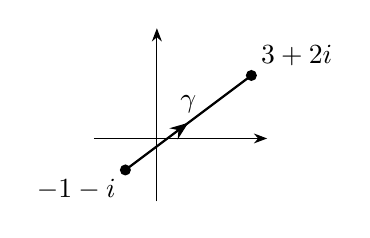
\begin{tikzpicture}[x=0.4cm,y=0.4cm]
      \draw [-{Stealth}] (-2,0) -- (3.5,0);
      \draw [-{Stealth}] (0,-2) -- (0,3.5);
      \fill (-1,-1) circle (2pt) node [below left] {$-1-i$};
      \fill (3,2) circle (2pt) node [above right] {$3+2i$};
      \draw [postaction={decorate},decoration={markings,mark=at position .5 with {\arrow{Stealth}}},thick] (-1,-1) -- (3,2) node [midway,above] {$\gamma$};
    \end{tikzpicture}
  \end{center}
  積分路のパラメーター表示を
  \[\gamma(t)=(-1-i)(1-t)=(3+2i)t=(4+3i)t-1-i\]
  とおくと,
  \begin{align*}
    \int_\gamma z^2dz
    &=\int_0^1 \gamma(t)^2\gamma'(t)dt \\
    &=\int_0^1 ((4+3i)t-1-i)^2\cdot(4+3i) dt \\
    &=-\frac{11}{3}+16i
  \end{align*}
  となります(途中の計算は省略しました).
\end{example}

\begin{example}
  関数 $f(z)=\frac{1}{z}$ を $1$ から $-1$ まで,2通りの積分路(図の壱と弐)で積分してみましょう.
  この関数は $z=0$ で定義されないので,積分路は $z=0$ を通らないように選ぶ必要があります.

  \begin{center}
    \begin{tikzpicture}
      \draw [-{Stealth}] (-2,0) -- (2,0);
      \draw [-{Stealth}] (0,-2) -- (0,2);
      \fill (-1,0) circle (2pt) node [above left] {$-1$};
      \fill (1,0) circle (2pt) node [above right] {$1$};
      \node [draw=black,cross out] at (0,0) {};
      %\draw (-2pt,-2pt) -- (2pt,2pt) (2pt,-2pt) -- (-2pt,2pt);
      \node (0,0) [above right] {$0$};
      \begin{scope}[decoration={markings,mark=at position .5 with {\arrow{Stealth}}},thick]
        \draw [postaction={decorate}]
          (1,0) arc [start angle=0, end angle=180, radius=1]
          node [midway,above left] {壱};
        \draw [postaction={decorate}] (1,0) arc [start angle=0, end angle=-180, radius=1]
          node [midway,below right] {弐};
      \end{scope}
    \end{tikzpicture}
  \end{center}

  壱($z=0$ の上側を通る):
  $\gamma(t)=e^{\pi i t}$
  \[
  \int_\gamma \frac{dz}{z}
  =\int_0^1 \frac{\pi i e^{\pi i t}}{e^{\pi i t}} dt
  =\int_0^1 \pi i dt
  =\pi i
  \]

  弐($z=0$ の下側を通る):
  $\gamma(t)=e^{-\pi i t}$
  \[
  \int_\gamma \frac{dz}{z}
  =\int_0^1 \frac{-\pi i e^{-\pi i t}}{e^{-\pi i t}} dt
  =-\int_0^1 \pi i dt
  =-\pi i
  \]

  始点と終点が同じでも,積分路の違い($z=0$ の上側を通るか下側を通るか)によって積分の値が変わるのが分かります.
\end{example}

\begin{wrapfigure}{r}{3cm}
  \vspace*{-\intextsep}
  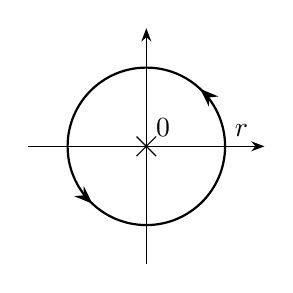
\begin{tikzpicture}
    \draw [-{Stealth}] (-1.5,0) -- (1.5,0);
    \draw [-{Stealth}] (0,-1.5) -- (0,1.5);
    \node at (1,0) [above right] {$r$};
    \node [draw=black,cross out] at (0,0) {};
    %\draw (-2pt,-2pt) -- (2pt,2pt) (2pt,-2pt) -- (-2pt,2pt);
    \node at (0,0) [above right] {$0$};
    \draw [postaction={decorate},decoration={markings,
        mark=at position .13 with {\arrow{Stealth}},
        mark=at position .63 with {\arrow{Stealth}}
    },thick]
      (1,0) arc [start angle=0, end angle=360, radius=1];
  \end{tikzpicture}
\end{wrapfigure}

積分路 $\gamma$ が半径 $r$ の円周 $\gamma(t)=re^{2\pi\ImagI t}$ の場合は,$\int_\gamma f(z)dz$ のことを
\[\int_{\abs{z}=r} f(z)dz\]
と書くことも多いです.向きは,特に断らない限り反時計回り(「正の向き」)に取ります.


\begin{example} \label{example:integrate-z^k}
  整数 $k$ について,$f(z)=z^k$ を原点の周りで(反時計回りに)一周するように積分してみます.
  %積分路は $\gamma(t)=e^{2\pi i t}$ とおきます.
  \[
  \int_{\abs{z}=r} z^k dz=\begin{cases}
  0 & k\ne -1 \\
  2\pi i & k=-1
  \end{cases}
  \]
  この積分値は積分路の半径 $r$ によらないこと,$k=-1$ の場合を覗くと積分値は $0$ となることがわかります.
\end{example}

\Section{コーシーの定理}
正則関数の積分について,次の重要な定理が成り立ちます.

\begin{theorem}[Cauchy]
  $f$ が $\Complex$ の単連結領域 $D$ で正則ならば,$D$ 内の区分的に滑らかな閉曲線 $\gamma$ について
  \[\int_\gamma f(z)dz=0.\]
\end{theorem}

「単連結」って何だよ!と思った人のために一言補足しておくと,単連結というのは内部に穴などが空いてない,ぐらいの意味です.
例えば,複素平面は単連結ですが,複素平面からいくつかの点を取り除くと単連結ではなくなります.
%複素平面から1点を取り除いた領域 $\Complex\setminus\{0\}$ で定義された関数 $f(z)=\frac{1}{z}$ についてコーシーの定理が成り立たないのは,\autoref{example:integrate-z^k} の通りです.
%複素平面や円板は単連結ですが,そこからいくつか点を取り除くと単連結ではなくなります.

この定理を使うと,例えば,複素平面全体で正則な関数は,始点と終点を決めてやればあとは積分路によらず積分値が定まることがわかります.
また,ある領域上での正則関数なら,その領域を逸脱しない範囲で積分路を多少変形させてもよいことがわかります(下図の領域内で正則な関数なら,積分路を $\gamma$ としても $\gamma'$ としても積分の値は同じ).

\begin{center}
\pgfdeclarepatternformonly{custom north east lines}{\pgfqpoint{-1pt}{-1pt}}{\pgfqpoint{8pt}{8pt}}{\pgfqpoint{7pt}{7pt}}%
{
  \pgfsetlinewidth{0.2pt}
  \pgfpathmoveto{\pgfqpoint{0pt}{0pt}}
  \pgfpathlineto{\pgfqpoint{7.1pt}{7.1pt}}
  \pgfusepath{stroke}
}
  \begin{tikzpicture}
    \draw [-{Stealth}] (-2,0) -- (2,0);
    \draw [-{Stealth}] (0,-1.8) -- (0,2);
    \draw [fill,pattern=custom north east lines] plot [smooth cycle, tension=1] coordinates {(-1.5,-0.9) (-0.3,-1) (1,-1.2) (1.6,0.3) (1.2,1.3) (0.1,1.1) (-1.1,1.2) (-1.5,0.3) (-1.5,-0.2)};
    \fill (-1,0) circle (2pt) node [above] {始点};
    \fill (1,0.2) circle (2pt) node [below=3pt] {終点};
    \draw [postaction={decorate},decoration={markings,mark=at position .58 with {\arrow{Stealth}}},thick]
      (-1,0) .. controls (0,-0.7) and (0.1,1.2) .. (1,0.2)
      node [midway,above left] {$\gamma$}
      ;
    \draw [postaction={decorate},decoration={markings,mark=at position .58 with {\arrow{Stealth}}},thick]
      (-1,0) .. controls (-0.4,-1.4) and (0.3,0.5) .. (1,0.2)
      node [midway,below right] {$\gamma'$}
      ;
  \end{tikzpicture}
\end{center}

\Section{留数}
関数 $f$ が $z=z_0$ を除いた領域で正則な時, $f$ は
%点 $z=z_0$ の除外近傍で正則な関数 $f$ を
\[f(z)=\dots+\frac{a_{-2}}{(z-z_0)^2}+\frac{a_{-1}}{z-z_0}+a_0+a_1(z-z_0)+a_2(z-z_0)^2+\dotsb\]
と展開できます.これを $f$ の $z=z_0$ におけるローラン(Laurent)展開と呼びます.

この $f$ を $z=z_0$ の周りで積分すると,\autoref{example:integrate-z^k} の結果より,
\begin{align*}
\int_{\abs{z-z_0}=r} f(z)dz
&=\int_{\abs{z-z_0}=r} \sum_{k=-\infty}^\infty a_k (z-z_0)^k dz \\
&=\int_{\abs{z-z_0}=r} \frac{a_k}{z-z_0} dz \\
&=2\pi i a_{-1}
\end{align*}
という風に,ローラン展開の $-1$ 次の係数(だけ)が出てきます.
この係数 $a_{-1}$ のことを, $f$ の $z_0$ での\ruby{留数}{りゅうすう}(residue)と呼びます.
正則関数を閉路に沿って積分する時,積分路の内部の特異点における留数が全部わかってしまえば,積分の値が決まってしまいます.

\begin{example}
  $f(z)=\frac{1}{z^3-1}$
  を考えます.
  この関数は,複素平面の $z=1,e^{2\pi i/3},e^{4\pi i/3}$ を除いた部分で定義された正則関数です.

  $f$ の $z=1$ におけるローラン展開は
  \[
  f(z)
  %=\frac{1}{(z-1)(z^2+z+1)}
  =\frac{1}{3}\frac{1}{z-1}+a_0+a_1(z-1)+\dotsb, %-\frac{1}{3}+\frac{2}{9}(z-1)+\dotsb,
  \]
  $z=e^{2\pi i/3}$ におけるローラン展開は
  \[
  f(z)
  =\frac{e^{2\pi i/3}}{3}\frac{1}{z-e^{2\pi i/3}}+a'_0+a'_1(z-e^{2\pi i/3})+\dotsb, %\frac{\sqrt{3}i}{9}+\dotsb,
  \]
  $z=e^{4\pi i/3}$ におけるローラン展開は
  \[
  f(z)
  =\frac{e^{4\pi i/3}}{3}\frac{1}{z-e^{4\pi i/3}}+a''_0+a''_1(z-e^{4\pi i/3})+\dotsb,
  \]
  となるので,それぞれの点における留数は $\frac{1}{3}$, $\frac{e^{2\pi i/3}}{3}$, $\frac{e^{4\pi i/3}}{3}$ です.

  この $f(z)$ を円周 $\abs{z}=2$ に沿って積分しましょう.
  この積分路の内部には3つの特異点が含まれます.
  \begin{center}
    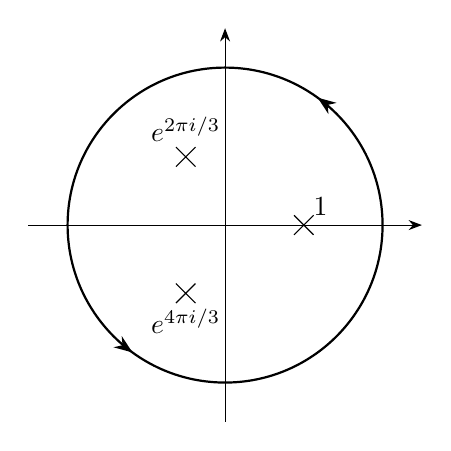
\begin{tikzpicture}
      \draw [-{Stealth}] (-2.5,0) -- (2.5,0);
      \draw [-{Stealth}] (0,-2.5) -- (0,2.5);
      \node [draw=black,cross out] at (1,0) {};
      \node [above right] at (1,0) {$1$};
      \node [draw=black,cross out] at (120:1) {};
      \node [above=2pt] at (120:1) {$e^{2\pi i/3}$};
      \node [draw=black,cross out] at (240:1) {};
      \node [below=2pt] at (240:1) {$e^{4\pi i/3}$};
      \draw [postaction={decorate},decoration={
          markings,
          mark=at position .15 with {\arrow{Stealth}},
          mark=at position .65 with {\arrow{Stealth}}
        },thick]
        (0,0) circle (2);
    \end{tikzpicture}
  \end{center}
  よって,この関数の $\abs{z}=2$ 上での積分は,内部の留数の和に $2\pi i$ をかけて,
  \[\int_{\abs{z}=2} f(z)dz=2\pi i\left(\frac{1}{3}+\frac{e^{2\pi i/3}}{3}+\frac{e^{4\pi i/3}}{3}\right)=0\]
  となります.
\end{example}


\Section{正則でない関数の例}

今までは「正則関数」,つまり複素数での意味の微分ができる関数を考えてきましたが,実数の意味での微分ができても複素数の意味での微分ができない関数というのも考えられます.
このような関数ではコーシーの定理は成り立たないので,複素積分をすると積分路の選び方によって積分の値が変わってしまいます.

\begin{example} \label{example:conjugate-integral}
  複素数にその共役を対応させる関数 $f(z)=\bar{z}$ を考えます.
  いくつかの積分路について,点 $0$ から点 $a+ib$ へ積分してみましょう.

  \begin{center}
    \begin{tikzpicture}[x=1.4cm,y=1.4cm]
      \draw [-{Stealth}] (-0.7,0) -- (2,0);
      \draw [-{Stealth}] (0,-0.7) -- (0,1.5);
      \fill (0,0) circle (2pt) node [above left] {$0$};
      \fill (1.3,1) circle (2pt) node [above right] {$a+ib$};
      \begin{scope}[thick]
        \draw [postaction={decorate},
               decoration={markings,mark=at position .5 with {\arrow{Stealth}}}
              ]
          (0,0) -- (1.3,1)
          node [midway,above left] {壱};
        \draw [
          postaction={decorate},
          decoration={
            markings,
            mark=at position .3 with {\arrow{Stealth}},
            mark=at position .8 with {\arrow{Stealth}}
          }
        ]
          (0,0) -- (1.3,0) -- (1.3,1)
          node [midway,right] {弐};
        \draw [
          postaction={decorate},
          decoration={
            markings,
            mark=at position .3 with {\arrow{Stealth}},
            mark=at position .8 with {\arrow{Stealth}}
          }
        ]
          (0,0) -- (0,1) -- (1.3,1)
          node [midway,above] {参};
      \end{scope}
    \end{tikzpicture}
  \end{center}

  なお,積分路が途中で折れ曲がっている場合は,積分路を適当に分割して足し合わせます.
  ここの例だと,弐と参はそれぞれ2つの線分に分割できるので,線分ごとにパラメーターをとって計算します.

  壱:
  $\gamma(t)=(a+ib)t$
  \[
  \int_\gamma f(z)dz
  =\int_0^1 (a-ib)t\cdot(a+ib)dt
  =\frac{a^2+b^2}{2}
  \]

  弐:
  $\gamma_1(t)=at$, $\gamma_2(t)=a+ibt$
  \begin{align*}
  \int_{\gamma_1+\gamma_2} f(z)dz
  &=\int_{\gamma_1} f(z)dz+\int_{\gamma_1} f(z)dz \\
  &=\int_0^1 at\cdot a dt+\int_0^1 (a-ibt)\cdot ib dt \\
  &=\frac{a^2}{2}+iab+\frac{b^2}{2}
  \end{align*}

  参:
  $\gamma_1(t)=ibt$, $\gamma_2(t)=at+ib$
  \begin{align*}
  \int_{\gamma_1+\gamma_2} f(z)dz
  &=\int_{\gamma_1} f(z)dz+\int_{\gamma_1} f(z)dz \\
  &=\int_0^1 (-ibt)\cdot ib dt+\int_0^1 (at-ib)\cdot a dt \\
  &=\frac{b^2}{2}+\frac{a^2}{2}-iab
  \end{align*}

  このように,3つの積分路で積分したものがどれも積分の値が異なっています.
\end{example}

\begin{exercise}
  \autoref{example:conjugate-integral} と同じ $f(z)=\bar{z}$ を,以下の閉じた積分路でそれぞれ積分せよ.

  \begin{enumerate}
  \item 長方形.
    \begin{center}
      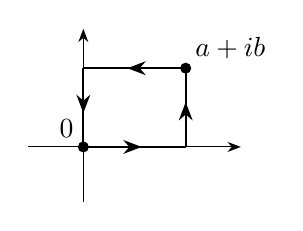
\begin{tikzpicture}
        \draw [-{Stealth}] (-0.7,0) -- (2,0);
        \draw [-{Stealth}] (0,-0.7) -- (0,1.5);
        \fill (0,0) circle (2pt) node [above left] {$0$};
        \fill (1.3,1) circle (2pt) node [above right] {$a+ib$};
        \begin{scope}[thick,
            decoration={markings,mark=at position .57 with {\arrow{Stealth}}},
            postaction={decorate}
          ]
          \draw [postaction={decorate}] (0,0) -- (1.3,0);
          \draw [postaction={decorate}] (1.3,0) -- (1.3,1);
          \draw [postaction={decorate}] (1.3,1) -- (0,1);
          \draw [postaction={decorate}] (0,1) -- (0,0);
        \end{scope}
      \end{tikzpicture}
    \end{center}

  \item 半径 $r$ の円.
  \end{enumerate}
\end{exercise}

\section*{おまけ}

今回は「たのしい複素積分」というWebページの紹介および複素積分のさわりを紹介しましたが,以前の駒場祭・五月祭では「複素関数で遊ぼう」というWebアプリの紹介をやりました.
内容は以下のURLから参照できます.
または,運の良い方なら「複素関数で遊ぼう」でググって見つけられるかもしれません.

\begin{center}
  \url{http://d-poppo.nazo.cc/math/complex-functions/}
\end{center}


\begin{thebibliography}{9}
\bibitem{Ahlfors}
  L.V. Ahlfors, \emph{Complex Analysis}, McGraw-Hill, 初版 1953, 第3版 1979.
\bibitem{Ahlfors-ja}
  L.V. アールフォルス 著 / 笠原 乾吉 訳 『複素解析』 現代数学社
\bibitem{Ueno}
  上野 健爾 『複素数の世界』はじめよう数学3, 日本評論社, 1999年
\end{thebibliography}

\end{document}
